\documentclass[UTF8]{book}

\renewcommand{\title}{模板示例:基于混沌学理论的数字图像加密技术}

\usepackage[fontset=none,heading=true]{ctex}
\setCJKmainfont{宋体}[AutoFakeBold={2.5}]
\setCJKsansfont{黑体}[AutoFakeBold={2.5}]
\setmainfont{Times New Roman}
\setsansfont{Arial}
\usepackage{amsmath}
\usepackage{amssymb}
\usepackage{booktabs}
\usepackage{float}
\usepackage{multirow}
\usepackage{array}
\usepackage{titletoc}
\usepackage{fontspec}
\usepackage{subfiles}
\usepackage{txfonts}
\usepackage{booktabs}
\usepackage{makecell}
\usepackage{caption}
\usepackage{tabularx}
\usepackage{hyperref}

\setmainfont{Times New Roman}
\setsansfont{Arial}

\newcommand{\xiaochu}{\fontsize{30pt}{40pt}\selectfont}    % 小初, 1.5倍行距
\newcommand{\yihao}{\fontsize{26pt}{36pt}\selectfont}    % 一号, 1.4倍行距
\newcommand{\erhao}{\fontsize{22pt}{44pt}\selectfont}    % 二号, 1.5倍行距
\newcommand{\xiaoer}{\fontsize{18pt}{27pt}\selectfont}    % 小二, 1.5倍行距
\newcommand{\sanhao}{\fontsize{16pt}{24pt}\selectfont}    % 三号, 1.5倍行距
\newcommand{\xiaosan}{\fontsize{15pt}{22pt}\selectfont}    % 小三, 1.5倍行距
\newcommand{\sihao}{\fontsize{14pt}{21pt}\selectfont}    % 四号, 1.5倍行距
\newcommand{\banxiaosi}{\fontsize{13pt}{19.5pt}\selectfont}    % 半小四, 1.5倍行距
\newcommand{\xiaosi}{\fontsize{12pt}{18pt}\selectfont}    % 小四, 1.5倍行距
\newcommand{\dawuhao}{\fontsize{11pt}{11pt}\selectfont}    % 大五号, 单倍行距
\newcommand{\wuhao}{\fontsize{10.5pt}{15.75pt}\selectfont}    % 五号, 单倍行距
\newcommand{\xiaowu}{\fontsize{9pt}{9pt}\selectfont}    % 小五号, 单倍行距

\usepackage{graphicx}
\usepackage[a4paper,
%bindingoffset=1cm,
left=3.18cm,
right=3.18cm,
top=2.54cm,
bottom=2.54cm,
footskip=1.5cm,
twoside,
]{geometry}

\usepackage{pdfpages}

\usepackage{fancyhdr}
\fancypagestyle{plain}{
    \fancyhf{} % clear all fields
    \fancyhead[CE]{\title} 
    \fancyhead[CO]{\leftmark} 
    \fancyfoot[C]{\thepage}
    
    \renewcommand{\headrulewidth}{0.4pt} 
    \renewcommand{\footrulewidth}{0pt}
}
\fancyhf{} % clear all fields
\fancyhead[CE]{\title} 
\fancyhead[CO]{\leftmark} 
\fancyfoot[C]{\thepage}
\pagestyle{fancy}
\renewcommand{\headrulewidth}{0.4pt} 
\renewcommand{\footrulewidth}{0pt}

\usepackage{tocloft}      %必须这么写,否则会报错

\renewcommand\contentsname{目\quad 录}
\renewcommand\cftbeforetoctitleskip{-7.5pt}
\renewcommand\cftaftertoctitleskip{15pt}
\renewcommand\cfttoctitlefont{\sffamily\xiaosan}
\renewcommand\cftdot{…}
\renewcommand{\cftdotsep}{0}

\renewcommand{\cftchapleader}{\cftdotfill{-0.5}} %设置chapter条目的引导点间距
\renewcommand{\cftsecleader}{\cftdotfill{-0.5}}
\renewcommand{\cftsubsecleader}{\cftdotfill{-0.5}}
\renewcommand{\cftchapfont}{\sffamily\sihao}    %设置chapter条目的字体
\renewcommand{\cftchappagefont}{\rmfamily\sihao}
\renewcommand{\cftbeforechapskip}{7pt}   
\renewcommand{\cftsecfont}{\sffamily\xiaosi}    %设置section条目的字体
\renewcommand{\cftsecpagefont}{\rmfamily\xiaosi}
\renewcommand{\cftbeforesecskip}{6pt}
\renewcommand{\cftsubsecfont}{\rmfamily\xiaosi} %设置subsection条目的字体
\renewcommand{\cftsubsecpagefont}{\rmfamily\xiaosi}
\renewcommand{\cftbeforesubsecskip}{6pt}

\DeclareCaptionLabelSeparator{fullcolon}{\quad}
\captionsetup{labelsep=fullcolon,font={bf,small,singlespacing},format=hang}


\usepackage{pifont}
\renewcommand\thefootnote{\ding{\numexpr171+\value{footnote}}}

\usepackage{xpatch}
\usepackage{scrextend}
\deffootnote[1.5em]{1.5em}{1em}{\thefootnotemark\space}

\newcolumntype{Y}{>{\centering\arraybackslash}X}
\renewcommand{\tabularxcolumn}[1]{>{\small}m{#1}}

%\usepackage[super, square, comma, sort&compress]{natbib}
\usepackage[sort]{gbt7714}
\bibliographystyle{gbt7714-2005-numerical}

\usepackage{titlesec}
\usepackage{setspace}


\begin{document}

    \frontmatter
    \setmainfont{Times New Roman}
\setsansfont{Arial}
\setmonofont{Courier New}

\ctexset{
        chapter = {
            format={\sffamily\xiaosan},
            beforeskip={-20pt},afterskip={15pt},
            name={,}, number={\arabic {chapter}}
        },
        section = {
            format={\sffamily \sihao},
            %beforeskip={-7pt},afterskip={-7pt},
        },
        subsection = {
            format={\rmfamily\xiaosi},
            %beforeskip={0pt},afterskip={0pt},
        }
}

%\titlespacing{\chapter}{0pt}{7.5pt}{7.5pt}
\titlespacing{\section}{0pt}{19pt}{7pt}
\titlespacing{\subsection}{0pt}{3pt}{3pt}

\makeatletter
% cancel the superscript style of counter used in footnote text
\xpatchcmd\@makefntext
  {{\hss\@makefnmark}}
  {{\hss\@makefnmark@nosuperscript}\space}
  {}{}

% old: superscript style
% \def\@makefnmark{\hbox{\@textsuperscript{\normalfont\@thefnmark}}}

% new: normal style, lower baseline
\def\@makefnmark@nosuperscript{\hbox{\normalfont\@thefnmark}}
\makeatother
    \begin{titlepage}
    \begin{center}
        \vskip \stretch{4}
        
\includegraphics[width=5.8cm]{figure/xmu-flag.pdf}\\
        \vskip \stretch{4}
        {\xiaoer \bfseries \quad 本\quad 科\quad 毕\quad 业\quad 论\quad 文\quad (设\quad 计)\quad}\\
        \vskip \stretch{2}
        {\sanhao \bfseries (主修专业)}\\
        \vskip \stretch{3}
        \begin{spacing}{2.5}
        {\sffamily \erhao \title}
        \end{spacing}
        %\vskip \stretch{1}
        \begin{spacing}{2.0}
        {\sanhao \bfseries Template Example: Digital Image Encryption Technology Based on Chaos Theory}
        \end{spacing}
        \vskip \stretch{2}

        \vskip \stretch{1}
        {\sihao
            \begin{tabular}{rl} 
                姓\qquad 名: & 张三 \\
                学\qquad 号: & 22920190000000 \\
                学\qquad 院: & 信息学院 \\
                专\qquad 业: & 人工智能 \\
                年\qquad 级: & 2019级 \\
                校内指导教师: & 张三\quad 教授 \\
                校外指导教师: & 张三\quad 经理\\
            \end{tabular}%
        }
        \vskip \stretch{2}
        \rmfamily\sihao
        \vskip \stretch{5.5}
        二〇二二年五月二十六日
        \vskip \stretch{2}
    \end{center}
\end{titlepage}
    
\includepdf[pages=1]{frontmatter/blank.pdf}
    \pagenumbering{Roman}
    \thispagestyle{empty}
{\sanhao \bfseries \centerline{厦门大学本科学位论文诚信承诺书}}

{\sihao
    \vspace{21pt}

	本人呈交的学位论文是在导师指导下独立完成的研究成果。本人在论文写作中参考其他个人或集体已经发表的研究成果,
    均在文中以适当方式明确标明,并符合相关法律规范及《厦门大学本科毕业论文(设计)规范》。
	
	该学位论文为(数字图像处理)课题(组)的研究成果,获得
	(数字图像处理)课题(组)经费或实验室的资助,
	在(人工智能)实验室完成。
	
	本人承诺辅修专业毕业论文(设计)(如有)的内容与主修专业不存在相同与相近情况。
	
	\vspace{42pt}
	
	\rightline{学生声明(签名):\hspace*{4cm}}

	\rightline{年\hspace{28pt}月\hspace{28pt}日\hspace*{2cm}}
}	
    \setcounter{page}{2}
    \addcontentsline{toc}{chapter}{致谢}
    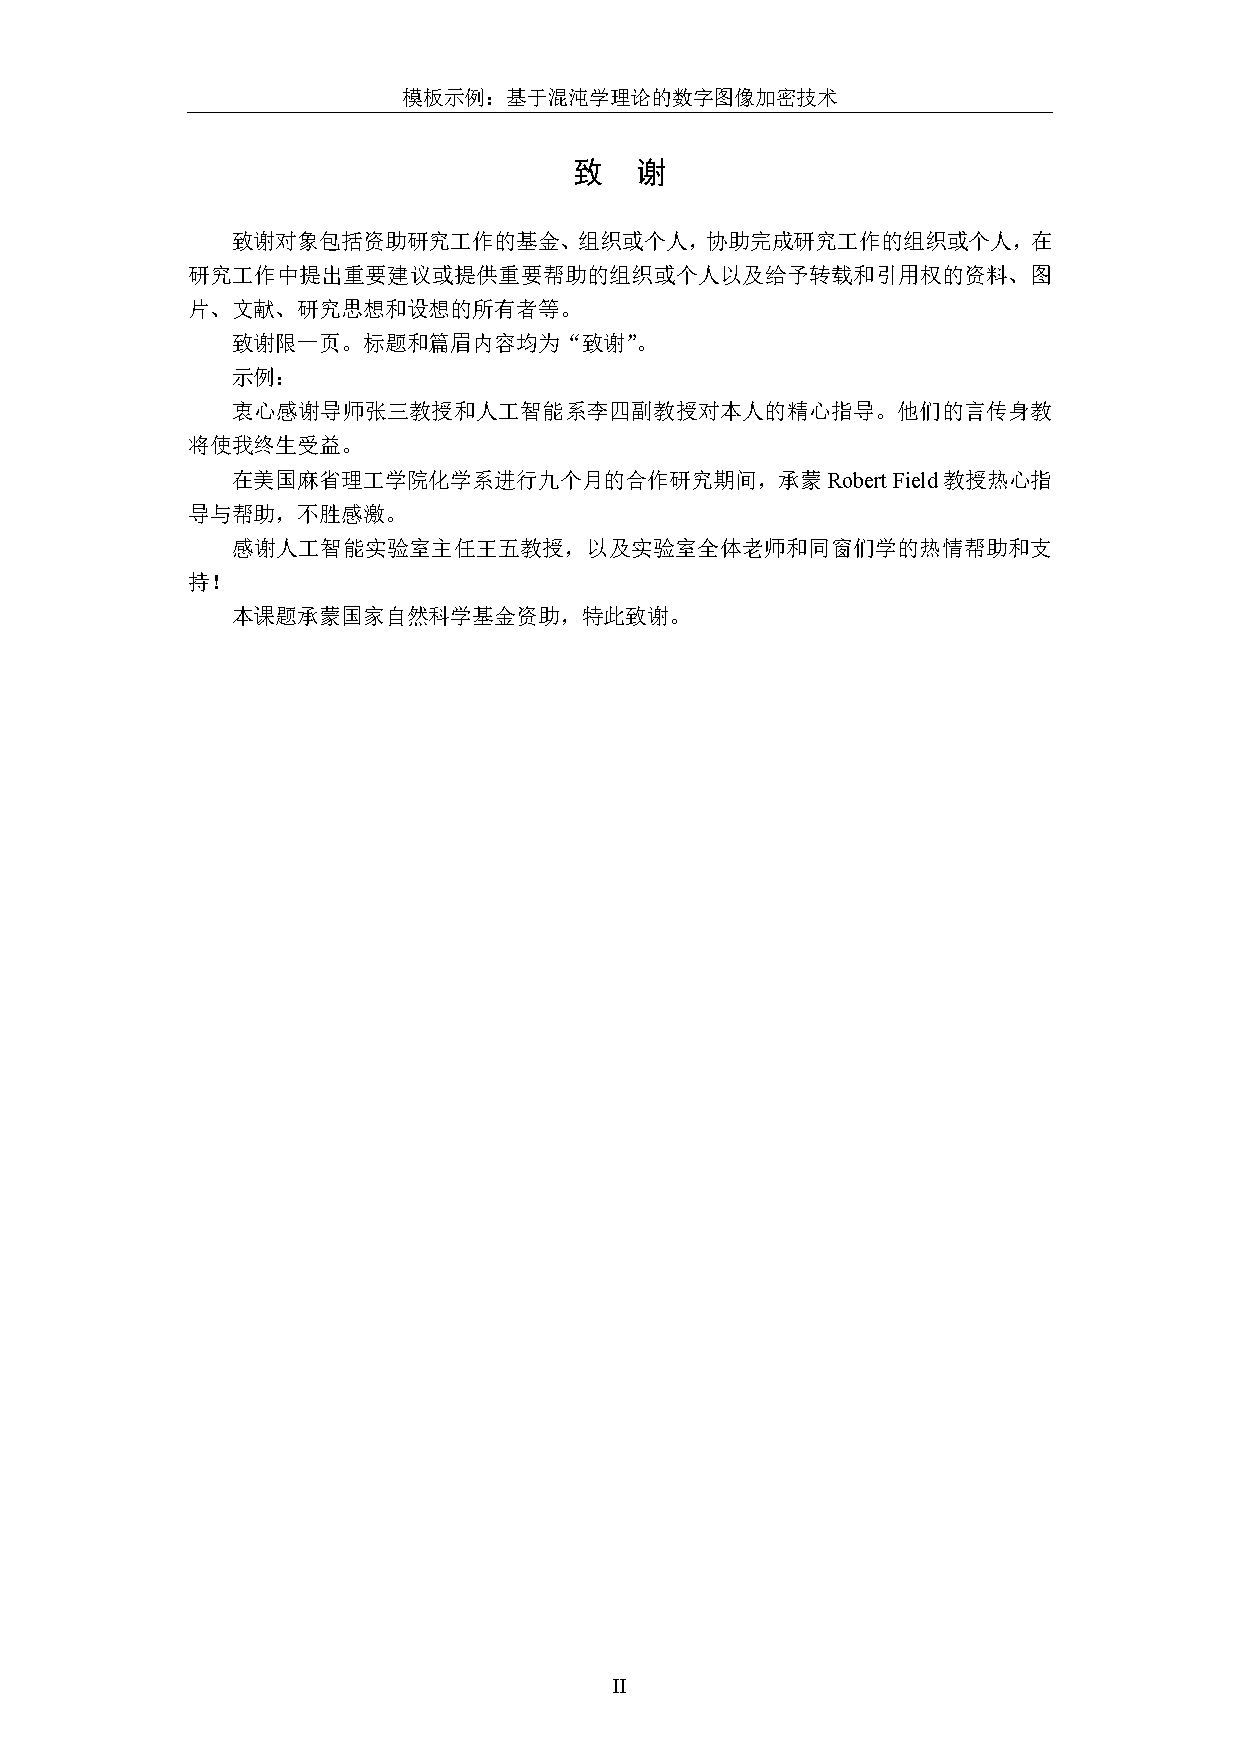
\includepdf[pages=1]{thanks_abstract.pdf}
    \setcounter{page}{3}
    \addcontentsline{toc}{chapter}{摘要}
    \includepdf[pages=2]{thanks_abstract.pdf}
    \setcounter{page}{4}
    \addcontentsline{toc}{chapter}{Abstract}
    \includepdf[pages=3]{thanks_abstract.pdf}
    \setcounter{page}{5}
    \addcontentsline{toc}{chapter}{目录}
    
\begin{center}\tableofcontents\end{center}

    \setcounter{page}{6}
    \addcontentsline{toc}{chapter}{Table of Contents}
    
\includepdf[pages=6]{content_en.pdf}
    

    \setmainfont{Times New Roman}
\setsansfont{Arial}
\setmonofont{Courier New}

\ctexset{
        chapter = {
            format={\sffamily\xiaosan},
            beforeskip={-20pt},afterskip={15pt},
            name={,}, number={\arabic {chapter}}
        },
        section = {
            format={\sffamily \sihao},
            %beforeskip={-7pt},afterskip={-7pt},
        },
        subsection = {
            format={\rmfamily\xiaosi},
            %beforeskip={0pt},afterskip={0pt},
        }
}

%\titlespacing{\chapter}{0pt}{7.5pt}{7.5pt}
\titlespacing{\section}{0pt}{19pt}{7pt}
\titlespacing{\subsection}{0pt}{3pt}{3pt}

\makeatletter
% cancel the superscript style of counter used in footnote text
\xpatchcmd\@makefntext
  {{\hss\@makefnmark}}
  {{\hss\@makefnmark@nosuperscript}\space}
  {}{}

% old: superscript style
% \def\@makefnmark{\hbox{\@textsuperscript{\normalfont\@thefnmark}}}

% new: normal style, lower baseline
\def\@makefnmark@nosuperscript{\hbox{\normalfont\@thefnmark}}
\makeatother    
    \mainmatter
    \chapter{引言}

近年来,图像加密一直是一个有吸引力的研究领域。它被广泛认为是一种用于安全传输的有用技术。
每个图像加密算法都旨在生成具有最高质量的嘈杂图像以保密信息。此外,图像加密对于保证网络上
的分类传输和图像容量具有较好的作用。随着互联网技术的飞速发展,数字通信变得更加广泛。人们
可以随时随地在互联网上发送数字图像。这导致了数字图像加密的发展。研究中表示数字图像加密的
不同方法与日益增加的安全必要性有关。基于混沌方法的图像加密是一种新颖的图像加密方法,它采
用随机混沌序列对图像进行加密,是解决高安全性和快速图像加密的棘手问题的有效途径。在过去的
几年里,出现了各种版本的混沌技术。目前,已采用四种方法进行图像加密,分别应用各种原理并实
现相同的目标。这四项原则包括共享和秘密分割、顺序排列、混沌动态系统和现代密码学,每项原则
都具有独特的特征。\citep{fu2012chaos}\par
本文的主要目的是提供一种基于混沌理论的数字图像加密新技术。它由 Y. Pourasad 等人提出。
然而,基于混沌的图像加密技术存在一些问题,包括准确性有限。为此,在本研究中,图像的加密
分为空间加密和变换域加密。在过去的几年里,一些图像加密方案被提出了频域和空间域。空间域
方法直接作用于普通图像的像素。\citep{yun2009digital, wang2008digital}由于这种方法包含高速加密,因此被广泛使用。使用变换域加密,
考虑到数字图像的一些典型属性,即高冗余和附近像素之间的强相关性。\par
本文以混沌序列和小波变换值以及图像加密算法的融合为导向。这种算法是通过分析算法来模拟的,
以发现差距。因此,算法得到了增强。该方法使用两个一维混沌系统,甚至可以使用基本非
线性方程来显示混沌行为。我们的主要目标,以及采用这种映射的比例,是发现一个新的离散时间
序列,与具有唯一参数的基本方程的逻辑映射的混沌输出相同。本文将在以下部分中介绍。在
“引言”部分,描述了问题的动机和陈述。此外,在“方法和材料”中,介绍了该方法的基本数学概念和
表达式。此外,在“提议的算法”部分,使用图形和表格描述了提议的模型实现的结果。此外,比较在
“算法”部分进行了介绍。最后,“结论”部分通过数值结果和透视概念总结了结果。\citep{yun2009digital, pourasad2021new}
    \chapter{材料与方法}
本章将介绍一些基于混沌理论的数字图像加密技术的理论知识,包括混沌理论、混沌随机序列和小波变换。
\section{混沌学概述}

混沌理论最早是由麻省理工学院的数学家和气象学家Edward Lorenz在 60 年代初的天气预报实验中发现的。
该理论即将探索明显随机数据中的隐藏模式。它提供了一种方便的方法来解决自然和人工系统的非线性问题,
这些系统具有不可预测的行为,例如道路交通、股票市场、地震、健康心脏的节律、DNA 编码序列、天气和
气候条件。对初始条件高度敏感的系统可以在混沌理论的保护伞下进行研究,混沌理论有意提及蝴蝶效应。
蝴蝶效应通常被解释为蝴蝶在巴西拍打翅膀并在德克萨斯州引发飓风。这意味着大系统中的微小变化可能会产
生复杂的结果。在这种情况下,该系统可能是从天气模式到小行星运动或人们的互动的任何东西,整个系统受
到影响的微小变化。从科学上讲,它被称为对初始条件 Dooley 的敏感依赖。由于计算中的一些数值错误,产
生了各种初始条件。这些误差为某些动态系统提供了大相径庭的结果。这使得几乎不可能预测长期渲染的行为。
即使系统的行为是由同一系统的初始条件决定的,并且过程中不涉及随机元素,也会发生这种情况。具有这种
条件的动态系统称为确定性系统。不足以使它们可预测的这种确定性行为的动态系统被标记为确定性。
因此,Edward Lorenz 尝试用一个单一的定义来描述混沌理论的主要概念。他说:“现在可以决定未来,但
大概的现在不能决定大概的未来”。这种预测随机性问题是一个巨大的问题。
\section{基于逻辑图的混沌序列}

显示二次非线性的一个离散时间维非线性系统称为逻辑图。逻辑图函数可以表示为:
\begin{equation}
    f(x)=\mu_{x}(1-x) \label{eq:logic graph function 1}
\end{equation}
状态方程的形式表示为:
\begin{equation}
    x_{n+1}=f(x_{n})=\mu_{x_{n}}(1-x_{n}) \label{eq:logic graph function 2}
\end{equation}
其中$x_{n}\in (0,1)$和$\mu\in (0,4)$被称为控制参数或分岔参数。\par
这里,$x_{n}$表示系统在$n$时间的状态。$x_{n+1}$表示下一时刻状态,$n$表示离散时间。
通过重复迭代关闭,增加了一系列点$\{x_{n}\}_\infty$,称为轨道。
逻辑图的性能对$\mu$的值很敏感。对于$\mu=3.574$,逻辑图是混沌的。
对于不同的初级条件,使用两个逻辑图来执行重复操作。此外,动态测量两个逻辑图的状态值。通过这个操作,产生了混沌序列。

\section{小波变换}

用于分析信号频率分量的一种有价值的仪器称为傅里叶变换。以傅立叶在整个时间轴上进行转换,
不可能确定增加特定频率的确切时刻。傅里叶变换和小波变换是相同的,具有完全不同的评价函数。
小波变换主要旨在仅通过变换时间扩展而不是形状来允许变化。两者的主要区别在于信号通过傅里
叶变换分解为余弦和正弦;然而,小波变换利用了傅里叶和实空间中的函数。通常,小波变换表述如下:
\begin{equation}
    f(a,b)=\int_{\infty}^{-\infty}f(x)\varPsi^*(a,b)\,\text{d}x \label{eq:wt}
\end{equation}
其中*代表复共轭符号,函数是一个函数,只要它遵循一定的规则,就可以任意选择。小波变换可以将信
号转换为时间、空间和频率作为独立的空间。它还侧重于任何局部细节的特定信号。因此,通过小波变换
可以有效地从信号中提取更多信息。\par
存在多种类型的小波变换用于特定目的。我们使用连续和离散小波变换从信号中提取更多信息。与傅里
叶变换类似,连续小波变换使用内积来测量信号和分析函数之间的相似性。理论分析是使用连续小波变
换的领域之一。在作为研究功能领域的计算机的特定实现中,必须对连续小波进行离散化。按照一些确
定的规则通过一组离散的小波尺度和平移运行小波变换称为离散小波变换。信号通过变换为相互正交的
小波群来分解,作为连续小波变换的必要变化。
此外,离散时间序列的实现有时被确定为离散时间连续小波变换。选择用于时频分解的小波是最重要的
一点。通过这种选择,我们可以影响结果的频率和时间分辨率。这种方式不能替代小波变换(WT)的基
本特征(低频具有错误的时间分辨率和真实频率;较高频率具有错误的频率分辨率和良好的时间)。然
而,以某种方式增加总时间分辨率的总频率是可能的。它与傅里叶和实空间中使用的小波宽度成正比。
使用 Morlet 小波,我们可以假设高频分辨率是频率中非常好的局部化小波。相反,利用高斯小波的导
数将导致正确的时间定位但频率较低。
    \chapter{算法}

本节可按小标题划分。
它应该对实验结果、它们的解释以及可以得出的实验结论提供简明准确的描述。
实施建议算法的步骤是:\\ \par

\noindent
\hangafter=1
\setlength{\hangindent}{4em}
步骤1:排列一张灰度图。图像的大小设置为$m\times n$。 
此外,放置了数据矩阵$R$。 通过评估两个逻辑图,生成一个混沌序列。 与主图像进行 XNOR,扩散终止。

\noindent
\hangafter=1
\setlength{\hangindent}{4em}
步骤2:本步骤中,对步骤1中的漫反射图像进行小波分解,提取小波系数,记为ca1。

\noindent
\hangafter=1
\setlength{\hangindent}{4em}
步骤3:利用二维超混沌图CML产生混沌序列,并利用步骤2中建立的ca1进行位置混淆。

\noindent
\hangafter=1
\setlength{\hangindent}{4em}
步骤4:在最后一步,可以通过小波重建混淆图像,得到了加密的图像。加密的逆运算称为解密算法。 图像加密和图像解密中的系统参数和混沌序列的初值是一致的。

\section{加密评估指标}

我们通过选择一些基本参数来评估算法来衡量我们的密码方案的性能。视觉检查是评估加密图像的主要参数之一。
特征扩散调查是判断随机化算法的另一个参数。通过检查,确定产品与一组确定的特征的偏差。人工操作通常完成
检查;然而,机器视觉被用于自动化这个过程。由于算法的良好扩散,原始图像和加密图像之间的关联变得过于复
杂,无法简单地预测。在这里,我们研究了峰值信噪比 (PSNR) 计算指标,即加密图像和关键图像之间的关联。
最终,我们通过计算统一平均变化强度 (UACI) 和像素数变化率 (NPCR) 两个参数来评估规范扩散。\citep{ul2020algebra}
\section{峰值信噪比 (PSNR)}

峰值信噪比 (PSNR) 是通过均方误差 (MSE) 确定的工程公式,它通常用于图像质量评估。公式如下\citep{xiao2009analysis}:
\begin{equation}
    \text{PSNR}=10\log \left(\frac{255^2}{\text{MSE}(f,f')}\right)
\end{equation}
其中$f(x,y)$和$f'(x,y)$表示原始图像和重建图像的像素值。
\section{像素数变化率 (NPCR)}

扩散以判断加密算法随机化的最基本参数的个数来表示。 
NPCRs 用于检查图像加密算法的安全性。
考虑$C_1$和$C_2$作为两个具有大小的图像,我们定义了一个与图像大小相似的数组:
\begin{equation}
    D(i,j)= \genfrac{\{}{}{0pt}{}{0,\, \text{if}\, C_1(i,j)=C_2(i,j)}{1,\, \text{if}\, C_1(i,j)\neq C_2(i,j)}
\end{equation}
NPCR 确定两个不同图像中像素的百分比,其计算公式如下\citep{wang2020image, wang2016novel, yun2009digital}:
\begin{equation}
    \text{NCPR}=\frac{\sum_{i}^{} \sum_{j}^{} D(i,j) }{N\times M}\times 100\%
\end{equation}
\section{统一平均变化强度 (UACI)}

UACI 使用以下表达式确定两个加密图像 ($C_1$和$C_2$) 内差异的平均强度,用于评估加密方法的强度,
它的值基于图像的格式和大小。 
通过 UACI,可以评估加密图像和原始图像之间的平均强度变化。 
最大的 UACI 表明所建议的技术对各种攻击具有抵抗力。 
UACI 的确定如下(假设灰度图像的大小为$M\times N$)\citep{ying2004digital}:
\begin{equation}
    \text{UACI}=\frac{1}{N\times M}\left[\sum_{i}\sum_{j}\frac{C_1(i,j)-C_2(i,j)}{\max(C_2)}\right]\times 100
\end{equation}
\section{数字图像关联 (DIC)}

数字图像相关 (DIC) 是一种关键且广泛使用的非接触式方法来测量材料变形。 
近年来,在开发新颖的实验 DIC 方法和提高相关计算算法的性能方面取得了重大进展。 
因此,加密图像和原始图像的相同像素之间的关系如下所示:
\begin{equation}
    \text{NC}=\sum_{m}\sum_{n}\frac{(A_{mn}-\overline{A})(B_{mn}-\overline{B})}{\sqrt{(A_{mn}-\overline{A})^2+(B_{mn}-\overline{B})^2} }
\end{equation}
其中$A$和$B$分别表示原始图像和加密图像,以及它们的均值。 
较低的相关系数值是最佳的。
    \chapter{实验和数值结果}

在本章中,我将使用 Y. Pourasad 等人的实验结果所提出的算法步骤的结果,如图 1 所示。
在第一步中,导入大小为$m\times n$的输入灰度图像。
基于图\ref{fig:4.1}\footnote{(顺带当作是脚注示例)注意给图片标签命名时不要像我这样使用4.1,
不然如果你要在前面加图片会导致很混乱,最好起别的名字},使用使用的两个逻辑图创建了一个混沌序列。
最后,在扩散步骤中,生成用于加密的安全密钥。
对于输入图像的加密,必须在小波分解子带之间插入安全密钥。 
DWT方法的子带如图\ref{fig:4.1}所示。DWT子带中从上到下和从左到右的图像是Low-Low、Low-High、High-Low和High-High子带。
利用二维超混沌映射 CML,产生混沌序列并进行混淆。
在最后一步,生成混淆图像。最后,图像由使用输入图像和安全密钥的加密矩阵组成。
用数值结果评估建议的算法表明该算法是稳健的。所提出算法的数值结果如表\ref{table:4.1}\footnote{
    注意给表格标签命名时不要像我这样使用4.1,
不然如果你要在前面加表格会导致很混乱,最好起别的名字(同样顺带当作是脚注示例)}所示。\\

\begin{figure}[ht]
    \begin{center}
        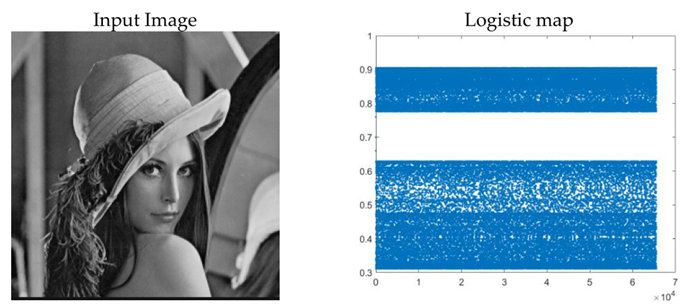
\includegraphics[width=\textwidth]{figure/p1.png}\\
        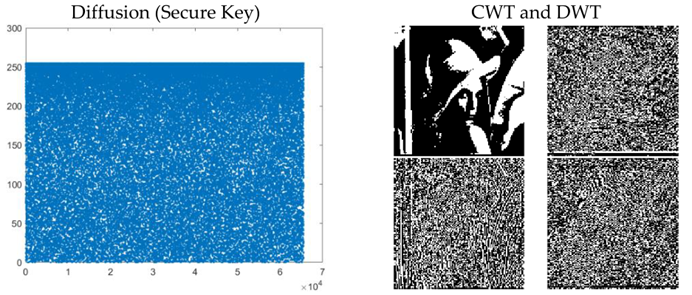
\includegraphics[width=\textwidth]{figure/p2.png}\\
        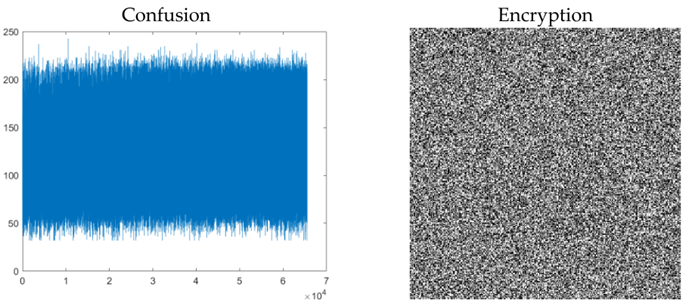
\includegraphics[width=\textwidth]{figure/p3.png}\\
    \end{center}
    \caption{所提出方法的处理结果 \label{fig:4.1}}
\end{figure}

\begin{table}[ht]
    \wuhao
    \caption{所提出的算法的数值结果 \label{table:4.1}}
    \begin{tabularx}{\textwidth}{YYYYYY}
        \Xhline{1.5pt}
        \bfseries Image & \bfseries Type & \bfseries PSNR & \bfseries NPCR & \bfseries UACI & \bfseries NC \\
        \Xhline{0.75pt}
        Lena & JPG & 42.612& 99.757 & 33.120 & 0.9548 \\
        Peppers & JPG & 39.220 & 99.787 & 33.621 & 0.9934 \\
        Barbara & JPG & 36.841 & 99.626 & 33.126 & 0.9809 \\
        Baloon & JPG & 39.134 & 99.881 & 33.415 & 0.9137 \\
        Boat & JPG & 39.223 & 99.625 & 33.671 & 0.9001 \\
        \Xhline{1.5pt}
    \end{tabularx}
\end{table}

首先,对原始图像(原始图像)进行扩散操作,主键值取自表\ref{table:4.2}。
 然后,在从表\ref{table:4.2}中获取主键值的同时执行混淆操作。 
 加密的结果与噪声相同(图\ref{fig:4.2})。 从加密图像中没有获取关于原始图像的信息。 
 通过对加密图像进行解密的密钥获取解密图像,然后进行扩散和混淆操作(图\ref{fig:4.2}(b))。\\

 \begin{table}[ht]
    \wuhao
    \caption{扩散和混淆操作的关键初始值 \label{table:4.2}}
    \begin{tabularx}{\textwidth}{YYYY}
        \Xhline{1.5pt}
        \bfseries Key (Diffusion) & \bfseries Value (Diffusion) & \bfseries Key (Confusion) & \bfseries Value (Confusion)\\
        \Xhline{0.75pt}
        $x_1(1)$ & 0.5 & $x_3(1)$ & 0.3 \\
        $x_2(1)$ & 0.5 & $y_3(1)$ & 0.3 \\
        $\mu_1$ & 4.0 & $\mu_1$ & 4.0 \\
        $\mu_2$ & 3.9 & $\mu_2$ & 3.9 \\
        \Xhline{1.5pt}
    \end{tabularx}
\end{table}

\begin{figure}[ht]
    \begin{center}
        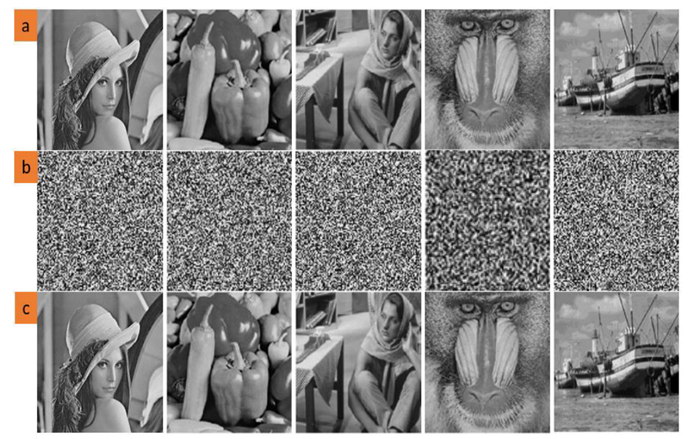
\includegraphics[width=\textwidth]{figure/p4.png}\\
    \end{center}
    \caption{将所提出的算法应用于某些图像的视觉结果\\ 
    (a) 原始图像; (b) 加密图像; (c) 重建图像 \label{fig:4.2}}
\end{figure}

\section{直方图分析}

第一个测试是加密、解密和原始图像的直方图分析。 
在这里,各个图像的图像直方图代表了加密图像和原始图像之间的巨大差异,但它们是相同的。 
通过对测试图像的直方图和加密后的直方图的评价,可以观察到加密后的图像在直方图的整个区间内是均匀分布的。 
因此,覆盖了原始图像的分布规律。 因此,有效地实施了加密(参见图\ref{fig:4.3})。

\begin{figure}[ht]
    \begin{center}
        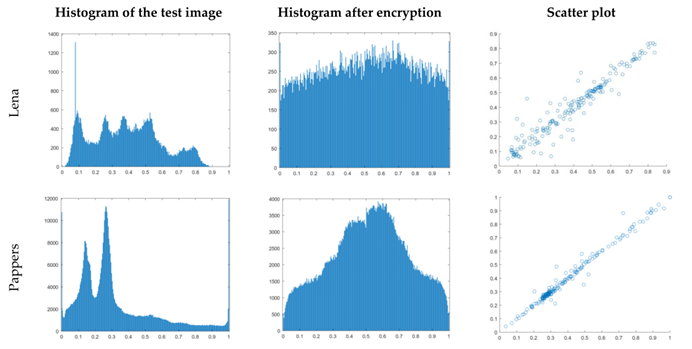
\includegraphics[width=\textwidth]{figure/p5.png}\\
        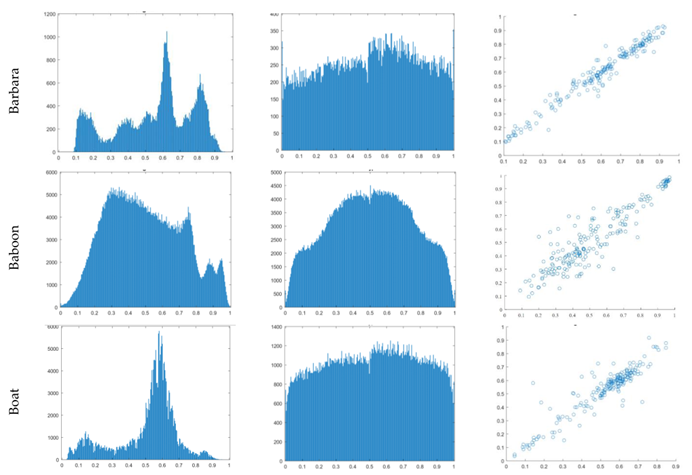
\includegraphics[width=\textwidth]{figure/p6.png}\\
    \end{center}
    \caption{原始 Lena 图像的直方图分析 \label{fig:4.3}}
\end{figure}
\section{鲁棒性 (健壮性)}

除了图\ref{fig:4.4} 中的直方图分析之外,Y. Pourasad等人还评估了输入图像和加密图像中两个垂直、
两个水平和两个对角相邻像素之间的相关性。 
图像中两个相邻像素的值由 x 轴和 y 轴表示。 
在输入图像和密码图像中,图\ref{fig:4.4}描绘了两个水平相邻像素的相关分布。 
普通图像和密码图像的相关系数分别为 0.99 和 0.02。 
对角线和垂直方向都产生相似的结果。 简单的图片具有两个相邻像素的高度相关性。

\begin{figure}[ht]
    \begin{center}
        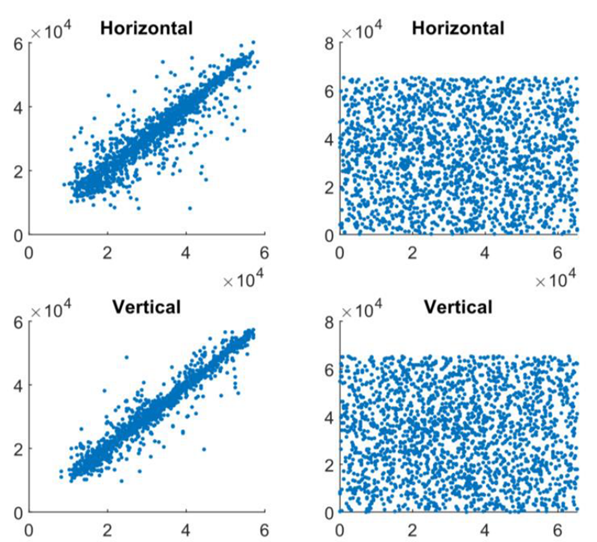
\includegraphics[width=\textwidth]{figure/p7.png}\\
        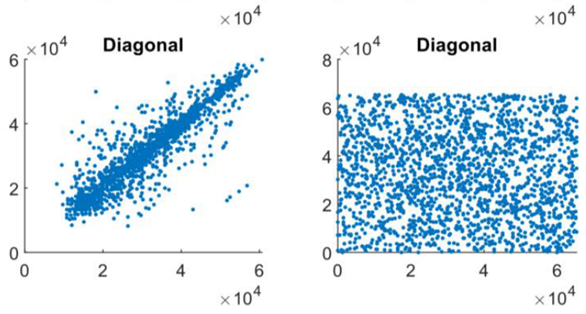
\includegraphics[width=\textwidth]{figure/p8.png}\\
    \end{center}
    \caption{Lena 图像中的像素水平、垂直和对角线、输入(左)和加密图像(右)的相关性图 \label{fig:4.4}}
\end{figure}

为了评估所提出的方法的鲁棒性,测试图像针对四种类型的图像处理攻击进行了测试:旋转、高斯噪声、中值过滤和直方图均衡。 
结果表明,所提出的设计具有更高的鲁棒性和归一化相关性。 根据结果,输入攻击不影响图像加解密。 关于不同类型图像的归
一化相关 (NC) 值,中值滤波器、旋转和高斯噪声具有更高的 NC 值。 这意味着所提出的方法的鲁棒性可以抵抗这些类型的攻
击。 然而,直方图均衡的影响是显着的(见表\ref{table:4.3})。\\

\begin{table}[ht]
    \wuhao
    \caption{所提算法在不同攻击类型下的 NC 值 \label{table:4.3}}
    \begin{tabularx}{\textwidth}{YYYYY}
        \Xhline{1.5pt}
        \bfseries Image & \bfseries Median Filter & \bfseries Histogram Equalization&\bfseries Rotation&\bfseries Gaussian Noise\\
        \Xhline{0.75pt}
        Lena & 0.984 & 0.987 & 0.999 & 0.999 \\
        Peppers & 0.704 & 0.280 & 0.923 & 0.964 \\
        Barbara & 0.914 & 0.497 & 0.980 & 0.991 \\
        Baloon & 0.960 & 0.629 & 0.991 & 0.996 \\
        Boat & 0.976 & 0.746 & 0.995 & 0.998 \\
        \Xhline{1.5pt}
    \end{tabularx}
\end{table}
    \chapter{结论}

最近,已经提出了各种基于混沌的图像密码系统。目前的工作是利用混沌映射和小波变换的特征来处理基于混沌的算法
该算法的加密过程包括两个阶段。首先,我们进行了图像扩散操作。此外,通过执行小波变换,由于超混沌序列而大大减少
了混淆计算量。标准度量的仿真结果表明,所提出的算法对密钥具有高度的依赖性。该算法包括一个不错的加密效果。
此外,它可以抵抗噪音和减少攻击。 Y. Pourasad 等人已经从基准 MATLAB 测试图像中测试了
Lena、Peppers、Barbara、Baboon 和 Boat 图像的提出方法。此外,还描述了输入图像和加密图像的直方图。
此外,还记录了PSNR、NPCR、UACI和NC等加密性能分析标准。根据结果​​,Lena、Peppers、Barbara、Baboon 
和 Boat 的相关值分别为 95.48\%、99.64\%、98.09\%、91.37\% 和 90.01\%。为了评估所提出的方法的鲁棒性,
测试图像针对四种类型的图像处理攻击进行了测试:旋转、高斯噪声、中值过滤和直方图均衡。结果表明,所提出的设
计具有更高的鲁棒性和归一化相关性。根据结果​​,输入攻击不影响图像加解密。关于不同类型图像的 NC 值,中值滤波、旋
转和高斯噪声具有更高的 NC 值。这意味着所提出的方法的鲁棒性可以抵抗这些类型的攻击。然而,直方图均衡的影响是显著的。
    %\backmatter
    
    \begin{center}
        \bibliography{backmatter/reference}
        \addcontentsline{toc}{chapter}{参考文献}
    \end{center}
    
\includepdf[pages=1]{frontmatter/blank.pdf} % 参考文献是奇数页的话请使用!
    \addcontentsline{toc}{chapter}{附录\space A\quad 关于本论文模板的相关说明}
    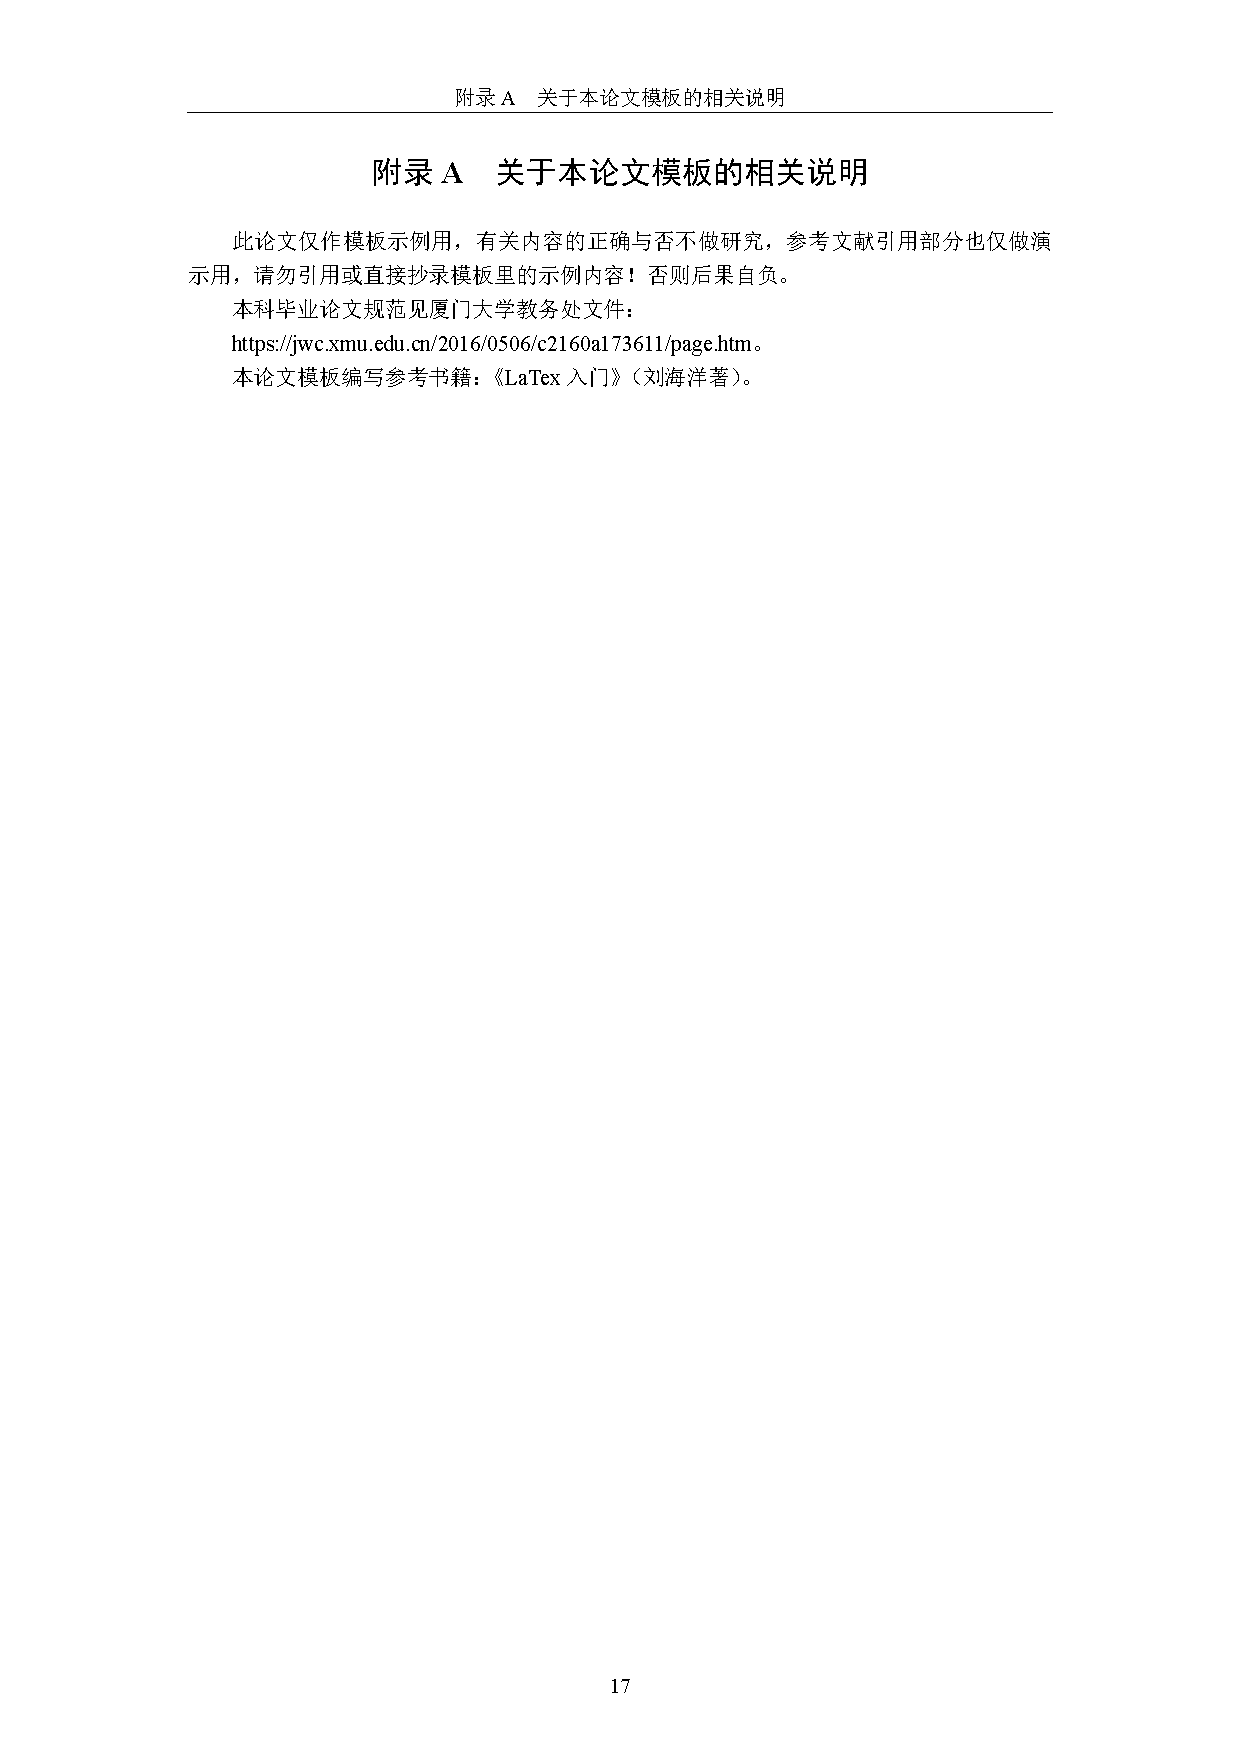
\includepdf[pages=1]{appendix.pdf}
    \addcontentsline{toc}{chapter}{附录\space B\quad 附录代码示例}
    \includepdf[pages=2-5]{appendix.pdf}
    
\end{document}